\documentclass[a4paper]{report}

\usepackage{natbib}
\usepackage{fancyvrb}
\usepackage{relsize}
\usepackage{graphicx}
\usepackage{amssymb,amsmath}
\usepackage{color}
\usepackage{hyperref}


\DefineVerbatimEnvironment{kappasource}{Verbatim}{baselinestretch=1,fontsize=\relsize{-1},commandchars=\\\{\}}
\DefineVerbatimEnvironment{bnfsource}{Verbatim}{baselinestretch=1,fontsize=\relsize{-1},commandchars=\\\{\}}
\DefineVerbatimEnvironment{pseudocode}{Verbatim}{baselinestretch=1,fontsize=\relsize{-1}}

\hypersetup{colorlinks=true,citecolor=blue,linkcolor=blue,urlcolor=blue}

\newcommand{\newbnf}[1]{\colorbox[rgb]{0.8,0.8,1}{#1}}

\title{Spatial Kappa Simulator\\User Guide\\v2.0.7}
\author{Donal Stewart\\DemonSoft.org}

\begin{document}

\maketitle

\section*{Acknowledgements}

The development of Spatial Kappa was funded in part by SynthSys. SynthSys is a Centre for Integrative Systems Biology (CISB) funded by BBSRC and EPSRC, reference BB/D019621/1.

\tableofcontents

\chapter{Spatial Kappa simulator User Guide}

\section{Obtaining the simulator}

The simulator is available from GitHub as the source Eclipse project, or as a single executable jar file. Both are available at \url{https://github.com/donal-s/SpatialKappa/downloads}. The simulator in its current state was optimised specifically for the 2010 Edinburgh iGEM project. This is apparent mostly in the design of the compartment view pane. Extending this view for more generic use is a planned extension.

\section{Starting the simulator}

\subsection{Running the executable jar}

The simulator can be started by running the executable jar file:\\
\verb|java -jar SpatialKappa-v1.0.0.jar|\\\\
Double clicking the jar file usually works too.

\subsection{Running from the Eclipse project}

The main class of the simulator is \\
\verb|org.demonsoft.spatialkappa.ui.TransitionMatchingSimulatorGui|\\\\
Running as a Java Application will bring up the simulator.


\section{Using the simulator}


The initial screen appears as figure \ref{fig:startup}.

\begin{figure}[h!]
 \centering
 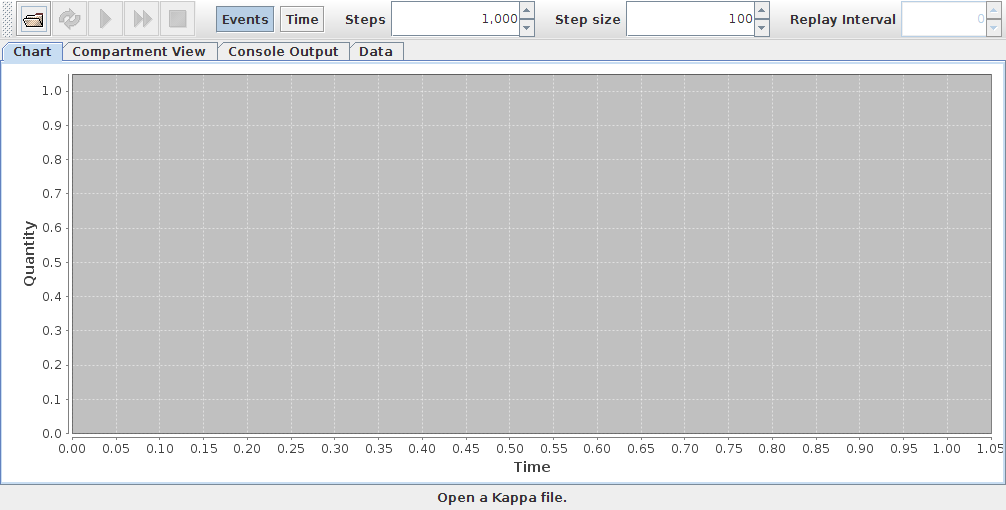
\includegraphics[scale=0.3]{./images/startup.png}
 % startup.png: 1006x510 pixel, 72dpi, 35.49x17.99 cm, bb=0 0 1006 510
 \caption{Initial view}
 \label{fig:startup}
\end{figure}

The toolbar options are:

\begin{tabular}{cl}
 
\includegraphics[scale=0.5]{./images/Open.png} & Open a Kappa or Kappa replay file \\
 
\includegraphics[scale=0.5]{./images/Reopen.png} & Reopen the current file  \\
 
\includegraphics[scale=0.5]{./images/Run.png} & Run the current file \\
 
\includegraphics[scale=0.5]{./images/Replay.png} & Replay the current replay file or last run \\
 
\includegraphics[scale=0.5]{./images/Stop.png} & Stop the currently running simulation \\
 
\includegraphics[scale=0.5]{./images/EventsOrTime.png} & Choose event or time based simulation \\
\end{tabular}

\subsection{Opening a Kappa or Kappa replay file}

Select the 'Open' button on the toolbar and select the file to open. The current implementation expects Kappa source files to have the suffix \verb|.ka| and Kappa replay files (discussed later) to have the suffix \verb|.kareplay|. If the file is parsed successfully, a summary of the Kappa model is displayed in the 'Data' pane (see figure \ref{fig:dataPane}). 

\begin{figure}[h!]
 \centering
 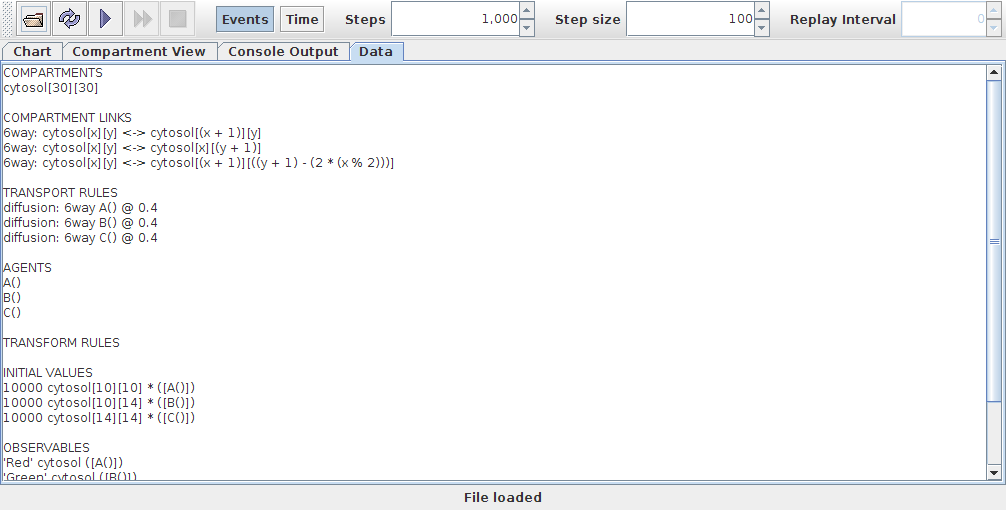
\includegraphics[scale=0.3]{./images/FileOpenDataPane.png}
 % FileOpenDataPane.png: 1006x510 pixel, 72dpi, 35.49x17.99 cm, bb=0 0 1006 510
 \caption{Data pane showing loaded Kappa model}
 \label{fig:dataPane}
\end{figure}

Any errors in reading the Kappa file are shown in the 'Console Output' pane.

The currently open Kappa file can be refreshed from disk by selecting the 'Reopen' button. Useful when editing the Kappa model.

\subsection{Running a simulation}

With a successfully opened Kappa model, one can run a simulation by selecting the 'Run' button. Simulation parameters can be set on the toolbar before running. There is the option to do an event or a time based simulation. For an event based simulation, the number of steps for the simulation (i.e. data points on the time series chart), and the number of finite rate events per step can be set. Equivalent options for time based simulation can also be set.

The simulation can be halted at any point by selecting the 'Stop' button. Note that complex simulations may take a while to start up while data structures are being generated.

\subsection{Running a simulation replay}

As the simulation runs, the state of the simulation observables are logged to disk in a replay file after every step. Once the simulation is complete, this replay file can be rerun by selecting the 'Replay' button. The 'Replay Interval' field allows a delay (in ms) to be added between each step.

Note - the current storage format is binary, and version dependent. Creation of a more permanent trace storage format is a planned enhancement.


\section{Spatial visualisation tools}

While the raw data produced from simulations is useful, visualisation of the data is important. There are a couple of simple visualisation panels in the simulator. These are dynamically updated as the simulation runs to give the user an idea of how the simulation is progressing. They are however basic in comparison to some of the commercial simulation data visualisation tools available.

The excellent JFreeChart \citep{JFreeChartwebsite} library was used for generating the charting components. Both charts have formatting and save capability, and the time series panel is zoomable.

\subsection{Time series chart}

This chart is similar to the standard Gnuplot output from Simplx. It is a line graph showing observable quantity against time for all observable definitions in the model.

\begin{figure}[h!]
 \centering
 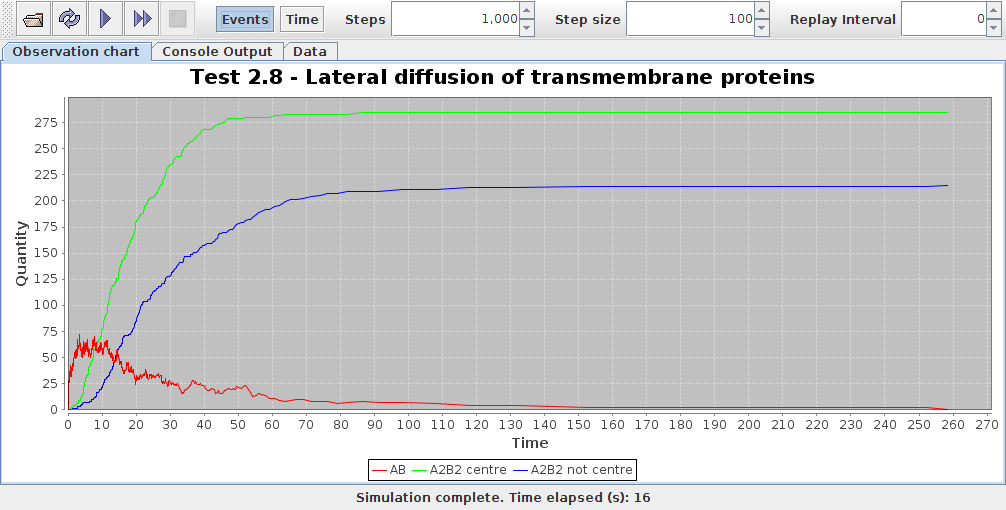
\includegraphics[scale=0.3]{./images/ChartPane.png}
 % ChartPane.png: 1006x510 pixel, 72dpi, 35.49x17.99 cm, bb=0 0 1006 510
 \caption{Sample time series chart output}
 \label{fig:chartPane}
\end{figure}

\subsection{Compartment chart}

This view allows more detailed visualisation of the transport of a species within the cells of a single compartment. It can show local positive feedback sites, or diffusion of a species through a compartment. There are a couple of visualisation options which can be selected at runtime to tailor the output.

Note that the current implementation is designed to view a 3-channel hexagonal mesh, and that view works only for observations labelled \verb|'Red'|, \verb|'Blue'| and \verb|'Green'| in a compartment labelled \verb|'Cytosol'|. Making this more generic is also a planned area for extension.

\begin{figure}[h!]
 \centering
 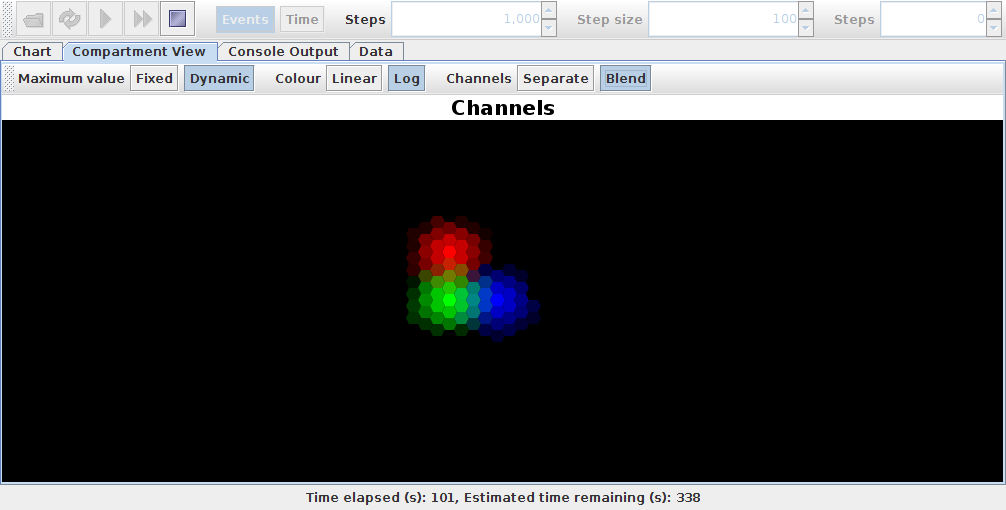
\includegraphics[scale=0.3]{./images/CompartmentView.png}
 % CompartmentView.png: 1006x510 pixel, 72dpi, 35.49x17.99 cm, bb=0 0 1006 510
 \caption{Sample compartment chart output}
 \label{fig:compartmentPane}
\end{figure}

\chapter{Kappa Language Extensions}

Note on terminology. In the following 'cell' can mean either a living cell, or a cell within a defined compartment. Hopefully the meaning in each situation will be clear from the context. Current Kappa rules are referred to as 'transform' rules as they cause some form of transformation of their substrates, be it change of agent state, agent creation or deletion, agent binding or unbinding. Species is mostly used to refer to a particular agent or complex in the model.

Also this document uses the terms 'language' and 'calculus' interchangeably, for example $\kappa$-calculus and Kappa language. Generally the term calculus is used when referring to the formal definition, and language where referring to models defined in Kappa, as they are represented in the Kappa language syntax.

\section{Existing Kappa language}

The current Kappa language consists of the following constructs, as described in the Simplx documentation \citep{krivine2009}. A more formal description of the language grammar (including the spatial extensions) is given in appendix \ref{chap:spatialGrammar}.

\textbf{Comments}:

\begin{kappasource}
# This is a comment
\end{kappasource} 

\textbf{Agents}:

\begin{kappasource}
AgentName()
AgentName(stateWithValue~stateValue, stateWithNoValue, unboundSite, boundSite!1)
\end{kappasource} 


\textbf{Transform rules}:

\begin{kappasource}
'state change' A(state~old) -> A(state~new) @ 0.1
'binding'      A(bindsite),B(bindsite) -> A(bindsite!1),B(bindsite!1) @ 0.1
'unbinding'    A(bindsite!1),B(bindsite!1) -> A(bindsite),B(bindsite) @ 0.1
'creation'     -> A() @ 0.1
'degradation'  A() -> @ 0.1
'reversible reaction'  A(state~old) <-> A(state~new) @ 0.1,0.2
A(state~old) -> A(state~new) @ 0.1 # Unnamed transform rule
\end{kappasource} 

\textbf{Initial species values}:

\begin{kappasource}
\%init 1000 * (A(state~old),C())            # 1000 of each of A(..) and C()
\%init 2000 * (A(bindsite!1),B(bindsite!1)) # 2000 of the bound complex A(..),B(..)
\end{kappasource} 

\textbf{Observables and named variables}: Variables can be referenced in perturbation calculations, but do not show in outputs as observations.

\begin{kappasource}
\%obs 'Label' A()  # All agents A()
\%obs A()          # Unnamed observation, will default to 'A()' in outputs
\%obs A(state~old) # All agents matching A(state~old)
\%obs 'binding'    # Activity of the transform rule named 'binding'

\%var 'Named variable' B()
\end{kappasource} 

\textbf{Perturbations}: These only fire a single time, after which they are disregarded for the rest of a simulation.

\begin{kappasource}
# When simulation time exceeds 5 seconds, change the rate of transform rule
#   named 'unbinding' to 10.0
\%mod: \$T > 5 do ’unbinding’:= 10.0

# When the species value mapped to observable 'mRNA' drops below 50
#   set the rate of transform named 'transcribe' to 0.5
\%mod: 'mRNA' < 50 do 'transcribe' := 0.5
\end{kappasource} 

\textbf{Currently unused}: There are some Kappa syntax elements not directly relevant to the spatial extensions, and will not appear in the extended grammar. One is a representation of causal flows, which uses the keyword \verb|%causal|.

\begin{kappasource}
\%causal: ’C@s2’ 
\%causal: {’A..B’,’C@s1’} => ’C@s2’ 
\end{kappasource} 


\section{Concepts to encapsulate}

The spatial Kappa language requires some encoding of the following concepts to be useful.

\begin{itemize}
 \item A description of \textbf{compartments} and their \textbf{dimensions}. A model may have multiple compartments each containing reacting species. The dimensions are necessary to define the shape of a compartment, be it a single cell, a 1 dimensional linear array of cells, a 2 dimensional grid of some form, or a 3 dimensional lattice structure. Relative differences in size of different compartments can be specified, e.g. the reacting volume of a nucleus relative to the surrounding cytosol. Relative differences in shape can also be specified, for example the thin layer of cytosol next to the inner surface of the plasma membrane versus the rest of the cytosol.

 \item A description of \textbf{linkage}, both intra-compartment and inter-compartment. The intra-compartment linkage specification should be rich enough to allow description of multiple structures, e.g. in 1D linear arrays or circles, in 2D square or hexagonal meshes, cylinders or tori, in 3D cubes, filled cylinders, spheres, etc.

 \item A means of \textbf{locating species} within compartments, e.g. all DNA would reside within the nucleus, or cell receptors would be limited to the plasma membrane.

 \item A means of \textbf{locating transform rules} within compartments, e.g. DNA transcription is isolated to the nucleus. The language should also allow the same transform rule to be specified with different rates depending on the location of the reacting species.

 \item A description of the \textbf{transport} (active or diffusive) of species within a compartment or between compartments along previously described linkage structures. The rates of transport should be general to all species, or species specific.

\end{itemize}


\textbf{Additional concepts}

\begin{itemize}
 \item \textbf{Granularity} within compartments. It would be useful to be able to specify locations at the level of compartments or single cells within a compartment. This would allow the model to represent, for example, a signal cascade being initiated as one point in the cytosol, and the resulting signal molecules being diffused through the cytosol. 

 \item \textbf{Backwards compatibility} with basic Kappa. Given the quantity of existing models, the extended language should allow the existing models to work as before without modification. The user should have the choice of not using the spatial aspects of the extended language with no rework penalty.

\end{itemize}


\section{New language constructs}

A full BNF description of the extended Kappa grammar is given in appendix \ref{chap:spatialGrammar}.

\subsection{Compartments and cells}

Compartments are defined as single cells or regular multidimensional arrays of cells as follows
\begin{bnfsource}
'\%compartment:' LABEL ('[' INT ']')*
\end{bnfsource}
For example
\begin{kappasource}
\%compartment: 'Single cell' 
\%compartment: '1d array' [10]       # 10 cells in size 
\%compartment: '2d array' [10][5]    # 10x5 cells in size 
\%compartment: '3d array' [10][5][4] # 10x5x4 cells in size 
\end{kappasource}

Compartments or individual cells within a compartment can be referenced using the following syntax
\begin{bnfsource}
LABEL ( '[' mathExpr ']' )*
\end{bnfsource}
where
\begin{bnfsource}
mathExpr :
  mathAtom OPERATOR mathAtom
  | mathAtom
  
mathAtom :
  '(' mathExpr ')'
  | INT
  | VARIABLE_NAME
  
OPERATOR :
  '+' | '-' | '*' | '/' | '\%'
\end{bnfsource}
For example
\begin{kappasource}
'my compartment'                     # the compartment as a whole
'my compartment' [0][0][0]           # the first cell in a 3d array compartment
'my compartment' [4]                 # the fifth cell in a 1d linear arrays

'my compartment' [x][y][z]           # variable name usage described in
'my compartment' [x*2][y-1][z+(x*3)] #   compartment links section below
\end{kappasource}

In all situations where compartment references are used, it is only legal to refer to the compartment as a whole by omitting the cell indices, or refer to a single cell, by fully defining the correct number of cell indices to match the dimensions of the compartment. Also, variable names are only permitted in compartment references within compartment link definitions, described below.

\subsection{Compartment links}

The structure of a compartment is further defined by how cells within the compartment are linked to each other and to connected compartments. This linkage is defined as follows
\begin{bnfsource}
'\%link:' LABEL compartmentReferenceExpr ('<->' | '<-' | '->') compartmentReferenceExpr
\end{bnfsource}
Where \verb|compartmentReferenceExpr| is as described above. For example
\begin{kappasource}
\%compartment: '2d array' [10][200]    # 10x200 cells in size 

# Link all cells to their horizontally adjacent neighbours
\%link: 'meshlinks' '2d array'[x][y] <-> '2d array'[x+1][y]

# Link all cells to their vertically adjacent neighbours
\%link: 'meshlinks' '2d array'[x][y] <-> '2d array'[x][y+1]

# Wrap around the cells on the left and right edges to create a cylinder
\%link: 'meshlinks' '2d array'[0][y] <-> '2d array'[9][y]

# Wrap around the cells on the top and bottom edges to create a torus
\%link: 'meshlinks' '2d array'[x][0] <-> '2d array'[x][199]
\end{kappasource}

The above code defines a thin torus composed of a 2d mesh.

Compartment references on the left hand side of the link definitions above may contain either constant values or single variable names, not complex expressions. The variable names are used to define the dimensions which will be iterated through to produce links. Compartment references on the right hand side allow constant values or complex expressions involving the variables defined on the left had side of the expression. It is invalid for the right hand expression to use variables not defined on the left. If setting the values of variables references valid cells on both the left and right, then those cells are deemed to be linked. References which refer to cells outside the dimensions of the compartment are ignored, and no link is created. The references in a link expression can refer to the same compartment, or two different compartments. The modulus operator \verb|%| is useful in defining regular, repeating linkage patterns within the compartment, for example the 2D hexagonal mesh described in appendix \ref{sec:spatialPatterns}.

Multiple link definitions can use the same label (like \verb|meshlinks| in the example above), in which case references to that label elsewhere in the model acts on the union of all the link definitions. This allows complex linkage definitions, for example compartments constructed in the form of a circle or sphere, to be referenced concisely in transport rules.

Further examples of compartment and link specifications for common structures are given in appendix
 \ref{sec:spatialPatterns}.

\subsection{Transport rules}

These rules define the rate at which species move from one compartment (or cell) to another.
\begin{bnfsource}
'\%transport:' (transportName=LABEL)? linkName=LABEL (agentGroup)? transportKineticExpr
\end{bnfsource}
  where
\begin{bnfsource}
agentGroup :
  agent (',' agent)*

transportKineticExpr :
  '@' a=rateValueExpr

rateValueExpr :
  number | '\$INF'   # \$INF means infinite rate
\end{bnfsource}

See appendix \ref{chap:spatialGrammar} for the definition of the remaining constructs. For examples of usage

\begin{kappasource}
# All species diffusing around the torus defined above
\%transport: 'general diffusion' 'meshlinks' @ 0.1

# Immediate exit of the named species through a uni-directional channel.
# Note the label for the transport is optional.
\%transport: 'Ca channel' Calcium() @ \$INF
\end{kappasource}

When referencing bidirectional compartment links (i.e. ones specified with '\verb|<->|', the rate applies equally in either direction across the link. In the second example above, care would need to be taken in defining the compartment link \verb|Ca channel| in the correct orientation.

\section{Additions to existing language constructs}

New clauses were added to existing Kappa language constructs to allow the use of compartments and links. In all cases, existing Kappa syntax is still valid. Where necessary, the optional label in existing Kappa statements is non-optional in statements using compartments to avoid ambiguity. When basic Kappa syntax is used in the context of a spatially aware model, the statement is generally taken to apply to all compartments in the model equally.

\subsection{Transform rules}

The following transform statement was added

\begin{bnfsource}
transformName=LABEL locationExpr transformExpr transformKineticExpr 
\end{bnfsource}
  where
\begin{bnfsource}
transformExpr :
  (a=agentGroup)? ( '->' | '<->' ) (b=agentGroup)?

transformKineticExpr :
  '@' a=rateValueExpr (',' b=rateValueExpr)?
\end{bnfsource}
For example
\begin{kappasource}
# mRNA degradation happens outside the nuclear membrane
'degradation' 'cytosol' mRNA() -> @ 6.21

# Heating of the agent occurs in cell 0 of the cytosol compartment
'heating' 'cytosol'[0] A(state~blue) -> A(state~red) @ 1.0
\end{kappasource}

As mentioned before valid locations are either entire compartments or single compartment cells.

\subsection{Initial values}

The following initial value statement was added

\begin{bnfsource}
initExpr :
  '\%init:' locationExpr INT '*' '(' agentGroup ')'
\end{bnfsource}
For example
\begin{kappasource}
# Distribute 2000 blue agents within the cells of cytosol equally
\%init: 'cytosol' 2000 * (A(state~blue)) 

# Add 500 red agents to cell 5 of the cytosol compartment
\%init: 'cytosol'[5] 500 * (A(state~red)) 
\end{kappasource}

\subsection{Observations}

The following observation statement was added

\begin{bnfsource}
obsExpr :
  '\%obs:' LABEL locationExpr agentGroup
\end{bnfsource}
For example
\begin{kappasource}
# Count all blue agents in all cells of the cytosol
\%obs: 'cytosol blue' 'cytosol' A(state~blue)

# Count all red agents in cell 0 of the cytosol compartment
\%obs: 'red[0]' 'cytosol'[0] A(state~red) 
\end{kappasource}


\bigskip For example models demonstrating the use of the language extensions, refer to appendix \ref{chap:resources}.

\newpage



\appendix
\chapter{Spatial Kappa Grammar}
\label{chap:spatialGrammar}



The following is a cut down version of the Antlr grammar used in the Kappa simulator. The syntax has been trimmed for readability, as the original Antlr grammar has artificial constructs for dealing with left recursion, etc. It is read basically as BNF notation with assignments (\verb|variable=bnfConstruct|). The existing basic Kappa grammar is shown in \verb|black|, with the spatial constructs shown as \SaveVerb{Verb}|blue| \newbnf{\UseVerb{Verb}}. 


\begin{bnfsource}
prog :
  (line)*

line :
  agentDecl NEWLINE!
  | \newbnf{compartmentDecl NEWLINE!}
  | \newbnf{channelDecl NEWLINE!}
  | ruleDecl NEWLINE!
  | initDecl NEWLINE!
  | plotDecl NEWLINE!
  | obsDecl NEWLINE!
  | varDecl NEWLINE!
  | modDecl NEWLINE!
  | COMMENT!
  | NEWLINE!

ruleDecl :
  label? transition rate 

transition :
  \newbnf{(source=location)? CHANNEL_TRANSITION channelName=id (target=location)?}
  | \newbnf{(a=agentGroup)? CHANNEL_TRANSITION channelName=id (b=agentGroup)?}
  | (a=agentGroup)? FORWARD_TRANSITION (b=agentGroup)?
  
agentGroup :
  \newbnf{location?} agent (',' agent)*

agent :
  id \newbnf{(location)?} ('(' (agentInterface (',' agentInterface)*)? ')')?

agentInterface :
  id state? link?

state :
  '~' id

link :
  '!' INT \newbnf{(':' channelName=id)?}
  | '!' '_' \newbnf{(':' channelName=id)?}
  | '?'

rate :
  '@' varAlgebraExpr

initDecl :
  '\%init:' (INT | label) agentGroup

agentDecl :
  '\%agent:' agentName=id ('(' (agentDeclInterface (',' agentDeclInterface)*)? ')')?

agentDeclInterface :
  id state*

\newbnf{compartmentDecl :}
  \newbnf{'\%compartment:' id ('[' INT ']')*}

\newbnf{channelDecl :}
  \newbnf{'\%channel:' linkName=id channel}
  \newbnf{| '\%channel:' linkName=id '(' channel ')' ('+' '(' channel ')')*}

\newbnf{channel :}
  \newbnf{source=locations FORWARD_TRANSITION target=locations}

\newbnf{locations :}
  \newbnf{location (',' location)*}

\newbnf{location :}
  \newbnf{':' sourceCompartment=id compartmentIndexExpr*}

\newbnf{compartmentIndexExpr :}
  \newbnf{'[' cellIndexExpr ']'}

plotDecl :
  '\%plot:' label

obsDecl :
  '\%obs:' label? agentGroup

varDecl :
  '\%var:' label varAlgebraExpr
   | '\%var:' label agentGroup

varAlgebraExpr :
  a=varAlgebraMultExpr (op=operator_add b=varAlgebraMultExpr )*
  
varAlgebraMultExpr :
  a=varAlgebraExpExpr (op=operator_mult b=varAlgebraExpExpr )*
  
varAlgebraExpExpr :
  a=varAlgebraAtom operator_exp b=varAlgebraExpExpr
  | a=varAlgebraAtom
  
varAlgebraAtom :
  '(' varAlgebraExpr ')'
  | number
  | label
  | '[' 'inf' ']'
  | '[' 'pi' ']'
  | '[' 'T' ']'
  | '[' 'E' ']'
  | operator_unary varAlgebraAtom
  | operator_binary_prefix a=varAlgebraAtom b=varAlgebraAtom
  
modDecl :
  '\%mod:' booleanExpression 'do' effect until?
  
booleanExpression :
  a=booleanAtom (op=booleanOperator b=booleanAtom )*
  
booleanOperator :
  '&&' | '||'

relationalOperator :
  '<' | '>' | '='

booleanAtom :
  '(' booleanExpression ')'
  | '[' 'true' ']'
  | '[' 'false' ']'
  | '[' 'not' ']' booleanAtom
  | a=varAlgebraExpr relationalOperator b=varAlgebraExpr

effect :
  '\$SNAPSHOT'
  | '\$STOP'
  | '\$ADD' varAlgebraExpr agentGroup
  | '\$DEL' varAlgebraExpr agentGroup
  | label ':=' varAlgebraExpr
  
until :
  'until' booleanExpression
  
\newbnf{cellIndexExpr :}
  \newbnf{a=cellIndexAtom operator_cell_index b=cellIndexAtom}
  \newbnf{| a=cellIndexAtom}
  
\newbnf{cellIndexAtom :}
  \newbnf{'(' cellIndexExpr ')'}
  \newbnf{| INT}
  \newbnf{| id}
  
id :
  ALPHANUMERIC ( ALPHANUMERIC | '_' | '-' )* 

label :
  LABEL

number :
  ( INT | FLOAT )
  
\newbnf{operator_cell_index :}
  \newbnf{( '+' | '*' | '-' | '/' | '\%' )}

operator_exp :
  | '^'

operator_unary :
  '[' 'log' ']'
  | '[' 'sin' ']'
  | '[' 'cos' ']'
  | '[' 'tan' ']'
  | '[' 'sqrt' ']'
  | '[' 'exp' ']'

operator_binary_prefix :
  '[' 'mod' ']'

operator_mult :
  '*' | '/'

operator_add :
  '+' | '-'

\newbnf{CHANNEL_TRANSITION :}
  \newbnf{'->:'}

FORWARD_TRANSITION :
  '->'

INT :
  NUMERIC

FLOAT :
  NUMERIC '.' NUMERIC EXPONENT?
  | '.' NUMERIC EXPONENT?
  | NUMERIC EXPONENT

ALPHANUMERIC :
  ( NUMERIC | 'a'..'z' | 'A'..'Z' )+

NUMERIC :
  ('0'..'9')+
  
EXPONENT :
  ('e'|'E') ('+'|'-')? NUMERIC

LABEL :
  '{\textbackslash}'' .* '{\textbackslash}''

COMMENT :
  '#' ~( '{\textbackslash}n' | '{\textbackslash}r' )*

NEWLINE :
  '{\textbackslash}r'? '{\textbackslash}n' | '{\textbackslash}r'

WS :
  ( ' ' | '{\textbackslash}t' | '{\textbackslash}{\textbackslash}' NEWLINE )+
\end{bnfsource}

\chapter{Spatial Kappa Examples}
\label{chap:resources}

\section{Spatial Kappa patterns}
\label{sec:spatialPatterns}

The following are generic shapes, with their equivalent Spatial Kappa representations. These are intended to be copied during model development.


\subsection{1 dimensional patterns}

\subsubsection{Linear array}

\begin{kappasource}
%compartment: array [n] # Replace n with length of array
%channel: intra-array (:array [x] -> :array [x+1]) + (:array [x] -> :array [x -1])
\end{kappasource}

\subsubsection{Circle}

\begin{kappasource}
%compartment: circle [n] # Replace n with number of cells in circle
%channel: intra-circle {\textbackslash}
    (:circle [x] -> :circle [x+1]) + (:circle [x] -> :circle [x -1]) + {\textbackslash}
    (:circle [n-1] -> :circle [0]) + (:circle [0] -> :circle [n -1]) # Replace n-1 as above
\end{kappasource}


\subsection{2 dimensional surfaces}

\subsubsection{Rectangular mesh}

There are 2 variants here, 4-way linked and 8-way linked.

\begin{kappasource}
%compartment: mesh [n][m] # Replace n and m with dimensions of mesh

# 4-way diffusion
%channel: intra-mesh {\textbackslash}
    (:mesh [x][y] -> :mesh [x+1][y]) + (:mesh [x][y] -> :mesh [x -1][y]) + {\textbackslash}
    (:mesh [x][y] -> :mesh [x][y+1]) + (:mesh [x][y] -> :mesh [x][y -1])

# or 8-way diffusion
%channel: intra-mesh {\textbackslash}
    (:mesh [x][y] -> :mesh [x+1][y]) + (:mesh [x][y] -> :mesh [x -1][y]) + {\textbackslash}
    (:mesh [x][y] -> :mesh [x][y+1]) + (:mesh [x][y] -> :mesh [x][y -1]) + {\textbackslash}
    (:mesh [x][y] -> :mesh [x+1][y+1]) + (:mesh [x][y] -> :mesh [x -1][y -1]) + {\textbackslash}
    (:mesh [x][y] -> :mesh [x+1][y -1]) + (:mesh [x][y] -> :mesh [x -1][y+1])
\end{kappasource}

These can also be specified using channel types as follows

\begin{kappasource}
%compartment: mesh [n][m] # Replace n and m with dimensions of mesh

# 4-way diffusion
%channel: intra-mesh EdgeNeighbour :mesh -> :mesh

# or 8-way diffusion
%channel: intra-mesh Neighbour :mesh -> :mesh
\end{kappasource}

\subsubsection{Hexagonal mesh}

Again, 2 variants depending on what overall shape is required. The first form has a simpler representation of intra-compartment links, but the overall structure is rhomboid, whereas the second produces an overall rectangular shape at the expense of more complicated link statements.

The second variant demonstrates handling of alternate odd-even linkage depending on the column of the structure.

\begin{kappasource}
%compartment: mesh [n][m] # Replace n and m with dimensions of mesh

# Variant 1 - rhomboid mesh
%channel: intra-mesh {\textbackslash}
    (:mesh [x][y] -> :mesh [x][y+1]) + (:mesh [x][y] -> :mesh [x][y -1]) + {\textbackslash}
    (:mesh [x][y] -> :mesh [x+1][y]) + (:mesh [x][y] -> :mesh [x -1][y]) + {\textbackslash}
    (:mesh [x][y] -> :mesh [x+1][y+1]) + (:mesh [x][y] -> :mesh [x -1][y-1])

# Variant 2 - rectangular mesh
%channel: intra-mesh {\textbackslash}
    (:mesh [x][y] -> :mesh [x][y+1]) + (:mesh [x][y] -> :mesh [x][y -1]) + {\textbackslash}
    (:mesh [x][y] -> :mesh [x+1][y]) + (:mesh [x][y] -> :mesh [x -1][y]) + {\textbackslash}
    (:mesh [x][y] -> :mesh [x+1][(y+1)-(2*(x%2))]) + {\textbackslash}
    (:mesh [x][y] -> :mesh [x -1][(y -1)+(2*((x -1)%2))])

# The above statement alternates [x+1][y+1] and [x+1][y-1] as x increases
\end{kappasource}

Variant 2 can also be specified using channel types as follows

\begin{kappasource}
%compartment: mesh [n][m] # Replace n and m with dimensions of mesh

# Variant 2 - rectangular mesh
%channel: intra-mesh Hexagonal :mesh -> :mesh
\end{kappasource}


\subsubsection{Cylinder and torus}

By connecting together the top and bottom edges of a mesh as described above, we get a cylinder. By also connecting together the left and right edges we get a torus.

\begin{kappasource}
%compartment: mesh [n][m] # Replace n and m with dimensions of mesh

# 4-way diffusion mesh
%channel: intra-mesh {\textbackslash}
    (:mesh [x][y] -> :mesh [x+1][y]) + (:mesh [x][y] -> :mesh [x -1][y]) + {\textbackslash}
    (:mesh [x][y] -> :mesh [x][y+1]) + (:mesh [x][y] -> :mesh [x][y -1])
%channel: intra-mesh mesh [x][y] <-> mesh [x+1][y] 
%channel: intra-mesh mesh [x][y] <-> mesh [x][y+1] 

# cylinder
%channel: intra-mesh {\textbackslash}
    (:mesh [x][y] -> :mesh [x+1][y]) + (:mesh [x][y] -> :mesh [x -1][y]) + {\textbackslash}
    (:mesh [x][y] -> :mesh [x][y+1]) + (:mesh [x][y] -> :mesh [x][y -1]) + {\textbackslash}
    (:mesh [x][y] -> :mesh [x][m -1]) + (:mesh [x][y] -> :mesh [x+1][0]) 
# Replace m-1 as above 

# torus
%channel: intra-mesh {\textbackslash}
    (:mesh [x][y] -> :mesh [x+1][y]) + (:mesh [x][y] -> :mesh [x -1][y]) + {\textbackslash}
    (:mesh [x][y] -> :mesh [x][y+1]) + (:mesh [x][y] -> :mesh [x][y -1]) + {\textbackslash}
    (:mesh [x][m -1] -> :mesh [x][0]) + (:mesh [x][0] -> :mesh [x][m -1]) + {\textbackslash}
    (:mesh [n -1][y] -> :mesh [0][y]) + (:mesh [0][y] -> :mesh [n -1][y])
# Replace n-1 as above 
\end{kappasource}

\newpage
\section{Sample Spatial Kappa models}

The following are a couple of simple spatial kappa models to demonstrate the use of the language features.



\subsection{2d diffusion model}
\label{sec:2dDiffusion}

This model shows simple diffusion from a point for three distinct species.


\begin{kappasource}
%agent: A()
%agent: B()
%agent: C()

%compartment: cytosol [30][30]

# 6-way diffusion
%channel: 6way {\textbackslash}
    (:cytosol [x][y] -> :cytosol [x][y+1]) + (:cytosol [x][y] -> :cytosol [x][y -1]) + {\textbackslash}
    (:cytosol [x][y] -> :cytosol [x+1][y]) + (:cytosol [x][y] -> :cytosol [x -1][y]) + {\textbackslash}
    (:cytosol [x][y] -> :cytosol [x+1][(y+1)-(2*(x%2))]) + {\textbackslash}
    (:cytosol [x][y] -> :cytosol [x -1][(y -1)+(2*((x -1)%2))])

'diffusion' ->:6way @ 0.4

%init: 10000 :cytosol[10][10] A
%init: 10000 :cytosol[10][14] B
%init: 10000 :cytosol[14][14] C

%obs: 'Red' A
%obs: 'Green' B
%obs: 'Blue' C
\end{kappasource}


\subsection{Bi-trivalent binding model}
\label{sec:bitrivalent}


A variant of bi-trivalent binding test model \citep{yang2008kinetic}. This spatial model allows unbound species to diffuse through the compartment, but bound species remain within a cell of the compartment.


\begin{kappasource}
%agent: A(a,b,bindings~0~1~2)
%agent: B(a,b,c)

%compartment: cytosol [20][20] 

# 6-way diffusion
%channel: 6way {\textbackslash}
    (:cytosol [x][y] -> :cytosol [x][y+1]) + (:cytosol [x][y] -> :cytosol [x][y -1]) + {\textbackslash}
    (:cytosol [x][y] -> :cytosol [x+1][y]) + (:cytosol [x][y] -> :cytosol [x -1][y]) + {\textbackslash}
    (:cytosol [x][y] -> :cytosol [x+1][(y+1)-(2*(x%2))]) + {\textbackslash}
    (:cytosol [x][y] -> :cytosol [x -1][(y -1)+(2*((x -1)%2))])

'diffusion-A' A(bindings~0) ->:6way A(bindings~0) @ 0.1 
'diffusion-B' B(a,b,c) ->:6way B(a,b,c) @ 1 

A(a,b,bindings~0), B(a) -> A(a!1,b,bindings~1),B(a!1) @ 1
A(a,b,bindings~0), B(b) -> A(a!1,b,bindings~1),B(b!1) @ 1
A(a,b,bindings~0), B(c) -> A(a!1,b,bindings~1),B(c!1) @ 1
A(a,b,bindings~0), B(a) -> A(a,b!1,bindings~1),B(a!1) @ 1
A(a,b,bindings~0), B(b) -> A(a,b!1,bindings~1),B(b!1) @ 1
A(a,b,bindings~0), B(c) -> A(a,b!1,bindings~1),B(c!1) @ 1
A(a,b!_,bindings~1), B(a) -> A(a!1,b!_,bindings~2),B(a!1) @ 1
A(a,b!_,bindings~1), B(b) -> A(a!1,b!_,bindings~2),B(b!1) @ 1
A(a,b!_,bindings~1), B(c) -> A(a!1,b!_,bindings~2),B(c!1) @ 1
A(a!_,b,bindings~1), B(a) -> A(a!_,b!1,bindings~2),B(a!1) @ 1
A(a!_,b,bindings~1), B(b) -> A(a!_,b!1,bindings~2),B(b!1) @ 1
A(a!_,b,bindings~1), B(c) -> A(a!_,b!1,bindings~2),B(c!1) @ 1

A(a!1,b,bindings~1),B(a!1) -> A(a,b,bindings~0), B(a) @ 0.01
A(a!1,b,bindings~1),B(b!1) -> A(a,b,bindings~0), B(b) @ 0.01
A(a!1,b,bindings~1),B(c!1) -> A(a,b,bindings~0), B(c) @ 0.01
A(a,b!1,bindings~1),B(a!1) -> A(a,b,bindings~0), B(a) @ 0.01
A(a,b!1,bindings~1),B(b!1) -> A(a,b,bindings~0), B(b) @ 0.01
A(a,b!1,bindings~1),B(c!1) -> A(a,b,bindings~0), B(c) @ 0.01
A(a!1,b!_,bindings~2),B(a!1) -> A(a,b!_,bindings~1), B(a) @ 0.01
A(a!1,b!_,bindings~2),B(b!1) -> A(a,b!_,bindings~1), B(b) @ 0.01
A(a!1,b!_,bindings~2),B(c!1) -> A(a,b!_,bindings~1), B(c) @ 0.01
A(a!_,b!1,bindings~2),B(a!1) -> A(a!_,b,bindings~1), B(a) @ 0.01
A(a!_,b!1,bindings~2),B(b!1) -> A(a!_,b,bindings~1), B(b) @ 0.01
A(a!_,b!1,bindings~2),B(c!1) -> A(a!_,b,bindings~1), B(c) @ 0.01

%init: 600 A(a,b,bindings~0) 
%init: 400 B(a,b,c) 

%obs: 'Red' A(bindings~2) 
%obs: 'Green' A(bindings~1) 
%obs: 'Blue' A(bindings~0) 
\end{kappasource}



\bibliographystyle{apalike}
\bibliography{SpatialKappaManual}

\end{document}
